%%%%
\section{Concentrações elementares}

No projeto global, envolvendo 11 pontos de amostragem em Acra, 
coletou-se 2898 amostras, todas analisadas na refletância e 
\textbf{Fluorescência de Raios X (XRF)} do 
\textbf{Laboratório de Análise dos Processos Atmosféricos - LAPAt} 
do \textbf{Instituto de Astronomia, Geofísica e Ciências Atmosféricas - IAG-USP}.

Os resultados gerais foram apresentados em 2011 no
\textbf{23th Congress of the International Society for Environmental 
Epidemiology} \citep{zhou2011} e publicados em \citep{zhou2013} e \citep{zhou2014}. 

Nesta pesquisa, em particular, aprofundou-se os estudos exclusivamente no bairro de Nima, 
com 791 amostras válidas coletadas em dois locais entre 11 de 
Novembro de 2006 e 15 de Agosto de 2008.

Os dois pontos de amostragem em Nima serão referidos como \textbf{residencial},
para medidas na rua só com residências e \textbf{avenida} para medidas na avenida
com presença de comércio e alto fluxo de veículos.

\begin{figure}[H]
\begin{center}
  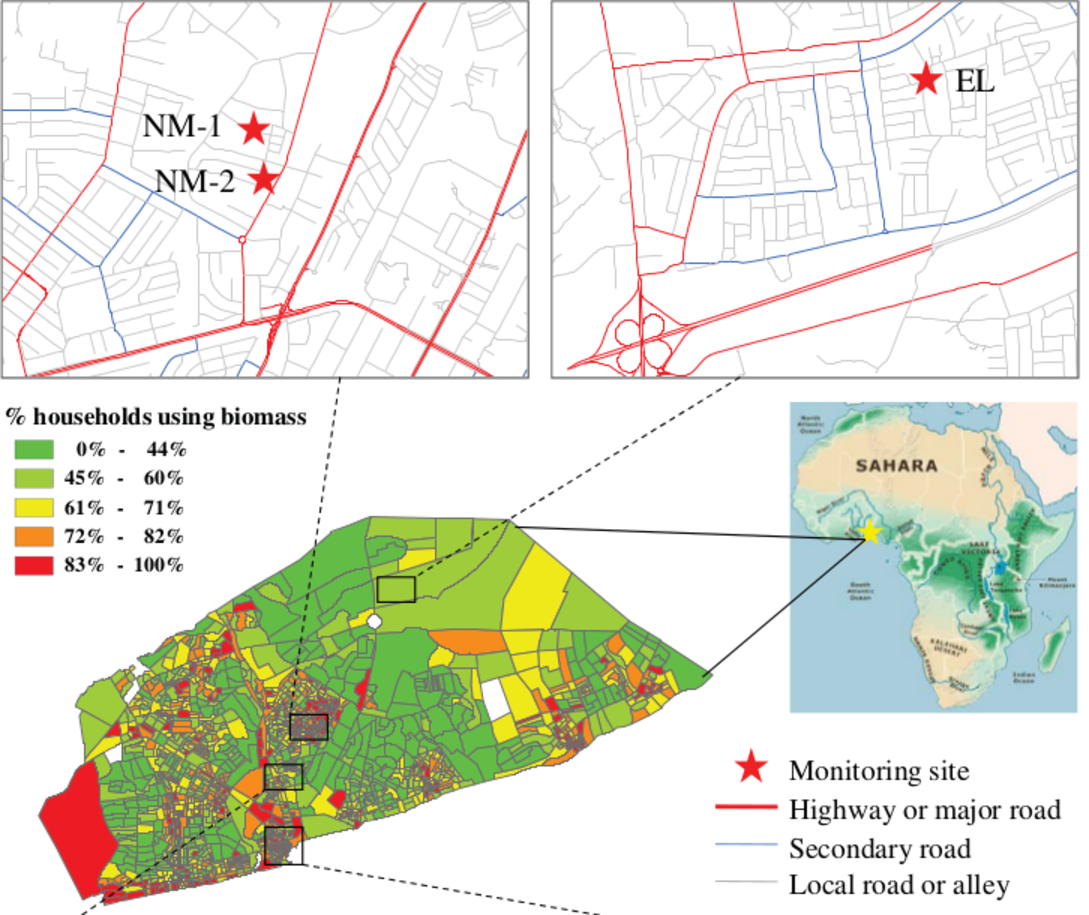
\includegraphics[width=0.6\textwidth]{../inputs/images/zheng/nima_mapa.pdf}
  \caption{Mapa de Nima. NM-1 ponto de amostragem na área residencial e 
           NM-2 ponto de amostragem na avenida. Porcentagem do uso da queima
           de biomassa para preparação de alimentos em residências usando dados
           do censo de 2000 \citep{ghanacensus2003} \label{fig:nima_mapa}}
\end{center}
\end{figure}


\begin{table}[H]
  \centering
  \begin{scriptsize}
  \input{../outputs/samples}
  \end{scriptsize}
  \caption{Quantificação total das amostras analisadas no \textbf{LAPAt}}
\end{table}

%\begin{table}[H]
% \centering
%  \begin{scriptsize}
%    \input{../outputs/tabela_descritiva_com_harmatan.tex}
%  \end{scriptsize} 
%  \caption{Média, desvio padrão e mediana da massa total e ultrapassagens das 
%           recomendações da Organização Mundial de Sáude (OMS) para média diária de 
%           25 $\mu g/m^3$ para $MP_{2,5}$ e 50 $\mu g/m^3$ para $MP_{10}$
%           \label{table:descritiva}}
%\end{table}

\begin{table}[H]
  \centering
  \begin{scriptsize}
    \input{../outputs/descriptive_RFcH}
  \end{scriptsize}
  \caption{Estatística descritiva para $MP_{2,5}$ na área \textbf{residencial}
           $\mu g / m^3$ \label{table:RFcH_descriptive}}
\end{table}

A média, desvio padrão da média, mediana, mínimo me máximo
A tabela \ref{table:RFcH_descriptive} traz as médias elementares de $MP_{2,5}$ na área 
\textbf{residencial}.
O \textbf{Black Carbon} representa $3,73 \%$ da massa total.



Média, desvio padrão e mediana da massa total e ultrapassagens das 
           recomendações da Organização Mundial de Sáude (OMS) para média diária de 
           25 $\mu g/m^3$ para $MP_{2,5}$ e 50 $\mu g/m^3$ para $MP_{10}$


Na tabela \ref{table:descritiva} estão as médias para a avenida e área residencial
bem como a porcentagem de ultrapassagem do padrão diário da 
Organização Mundial de Sáude (OMS).
O indíce de ultrapassagens foi alto para todos os casos, mas principalmente na avenida,
acima de (90\%) tanto para $MP_{10}$ quanto para $MP_{2,5}$.

Os padrões de qualidade do ar são fixados em níveis que quando ultrapassados 
podem afetar a saúde da população. 
Na tabela \ref{table:pm10standards} há uma comparação dos padrões de $MP_{10}$ 
no Brasil (CONAMA 03/90), Gana (EPA-Gana) e os recomentados pela Organização
Mundial de Sáude.
Outra recomendação da OMS é que a concentração não ultrapasse $25 \mu g/m^3$ 
em mais que 1\% das amostragens durante um ano. 

\begin{table}[H]
  \centering
  \begin{scriptsize}
    \input{../outputs/standard_brazil_ghana_OMS_pm10}
  \end{scriptsize}
  \caption{Padrões para $MP_{10}$ no Brasil (CONAMA 03/90), Gana (EPA-Gana) e 
          Organização Mundial de Sáude \label{table:pm10standards}}
\end{table}



%TODO: Fazer sem o harmatão e ver se BC aumenta.  
Já na avenida \ref{table:TFcH_descriptive} o \textbf{Black Carbon} 
representa 4.7 \% da massa total.

\begin{table}[H]
  \centering
  \begin{scriptsize}
    \input{../outputs/descriptive_TFcH}
  \end{scriptsize}
  \caption{Tabela com estística descritiva para $MP_{2,5}$ na \textbf{avenida}
          \label{table:TFcH_descriptive}}
\end{table}

No gráfico da figura \ref{fig:plot_RFcH_massa} percebe-se que no período 
do harmatão tanto o padrão nacional de Gana quanto a recomendação da OMS 
são ultrapassados.

%\begin{figure}[H]
%\begin{center}
%  \includegraphics[width=0.6\textwidth]{../outputs/plot_RFcH_massa.pdf}
%  \caption{Massa total $MP_{2,5}$ na área \textbf{residencial} \label{fig:plot_RFcH_massa}}
%\end{center}
%\end{figure}

%%%%
\subsection{Comparação dos resultados com dados da USEPA}

Verificação da qualidade dos resultado obtidos por XRF.
Entre as 2898 amostras analisadas por \textbf{ED-XRF}, existiam 92 que foram 
previamente analisadas pela \textbf{United States Environmental Protection 
Agency (USEPA)}, porém nós não sabíamos, pois o Prof. Dr. Majid Ezzati quis 
fazer um teste a cega das nossas medidas. 

Os elementos com concentrações muito acima do limite de detecção tiveram ótima
concordância, com pode ser observado no gráfico da figura \ref{fig:epa} 

\begin{figure}[H]
  \centering
    \includegraphics[width=0.3\textwidth]{../outputs/EPA_Si.pdf}
    \includegraphics[width=0.3\textwidth]{../outputs/EPA_Fe.pdf}
    \includegraphics[width=0.3\textwidth]{../outputs/EPA_P.pdf}
  \caption{Comparação das concentrações com análise da USEPA \label{fig:epa}.}
\end{figure}
